\chapter{Conceptual design}
First of all the structure itself of the received objects needs to be analyzed more in detail which are being provided by the \textbf{PCB-Investigator.exe}:\\

\begin{figure}[h]
	\centering
		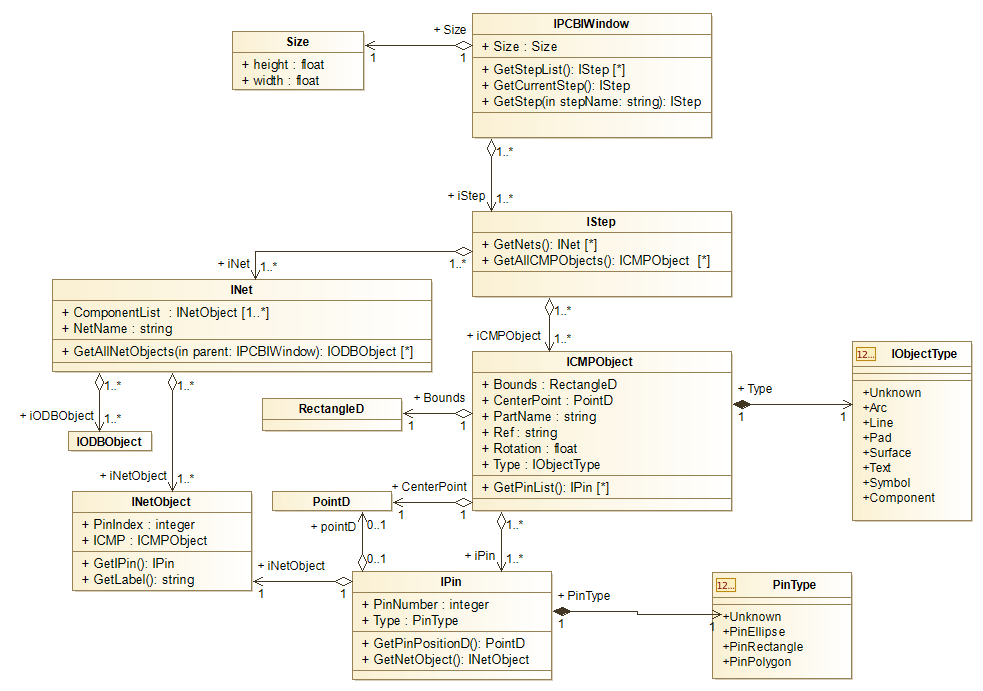
\includegraphics[width=1.00\textwidth]{figures/PCB Investigator class diagram.png}
	\caption{Class diagram of the PCB-Investigator objects of interest}
	\label{fig:PCB Investigator class diagram}
\end{figure}
As shown within \ref{fig:PCB Investigator class diagram} there could be seen that the very first class is the IPCBIWindow which contains a various amount of IStep objects. Within this IStep objects there are many INet objects and ICMPObjects. \newline
As ProMik GmbH is just interested in extracting all relevant information from any \ac{ODB}++ related projects the following public functions of the \textbf{PCB-Investigator.exe} where used by the created software\cite{.472021b} to extract all INet and ICMPObjects:

\begin{itemize}
	\item IAutomation.IAutomationInit() - Initialization of the \ac{API}
	\item IAutomation.CreateNewPCBIWindow(bool visible) - Creates the base window
	\item IPCBIWindow.LoadData(string path) - Loads a specific project into the window
	\item IPCBIWindow.GetStepList() - Getter for all steps of the window
	\item IStep.GetNets() - Getter for all nets of a step
	\item IStep.GetAllLayerNames() - Getter for all layer names of a step
	\item IStep.GetLayer(string layerName) - Getter for a layer in dependency on the layer name from a step
	\item ILayer.GetAllLayerObjects() - Getter for all objects which are located on a specific layer within a step
\end{itemize}